\documentclass[a4paper]{article}

\usepackage{INTERSPEECH2019}

\title{Disambiguation of Chinese Polyphones in an End-to-End Framework with Semantic Features Extracted by Pretrained BERT}
\name{Dongyang Dai$^{1, 2}$, Zhiyong Wu$^{1,2,3,*}$\thanks{* Corresponding author}, Shiyin Kang$^{4}$, Xixin Wu$^3$, Jia Jia$^{1,2}$, Dan Su$^{4}$, Dong Yu$^{4}$,\\Helen Meng$^{1,3}$}
%The maximum number of authors in the author list is twenty. If the number of contributing authors is more than twenty, they should be listed in a footnote or in acknowledgement section, as appropriate.
\address{
  $^1$Tsinghua-CUHK Joint Research Center for Media Sciences, Technologies and Systems, \\
  Graduate School at Shenzhen, Tsinghua University, Shenzhen, China\\
  $^2$Beijing National Research Centre for Information Science and Technology (BNRist),\\
  Department of Computer Science and Technology, Tsinghua University, Beijing, China \\
  $^3$Department of Systems Engineering and Engineering Management, \\
  The Chinese University of Hong Kong, Shatin, N.T., Hong Kong SAR, China\\
  $^4$Tencent AI Lab, Tencent, Shenzhen, China}
\email{ddy17@mails.tsinghua.edu.cn, \{zywu,wuxx,hmmeng\}@se.cuhk.edu.hk\\
	\{shiyinkang,dansu,dyu\}@tencent.com, jjia@tsinghua.edu.cn}

\begin{document}

\maketitle
% 
\begin{abstract}
  Grapheme-to-phoneme (G2P) conversion serves as an essential component in Chinese Mandarin text-to-speech (TTS) system, where polyphone disambiguation is the core issue. In this paper, we propose an end-to-end approach to predict the pronunciation of polyphonic character, which accepts sentence containing polyphonic character as input in the form of Chinese character sequence. The proposed method consists of a pretrained bidirectional encoder representations from transformers (BERT) model and a deep neural network (DNN) based classifier. The pretrained BERT model extracts semantic features from raw Chinese characters and the DNN classifier predicts the pronunciation of polyphonic character according to the extracted semantic features. Experimental results demonstrate that the proposed method outperforms the baseline approach which accepts word sequences encodes the contextual information with bidirectional long short-term memory (BLSTM) recurrent neural network using word sequence and part of speech (POS) sequence as input.
\end{abstract}

\noindent\textbf{Index Terms}: polyphone disambiguation, pretrained BERT, end-to-end framework

\section{Introduction}


Nowadays, Text to speech (TTS) techology has been widely applied in voice-assistants, car navigation, e-books and other products. The grapheme to phoneme (G2P) conversion component is essential in TTS system, which has a decisive influence on the quality of the synthesized speech. In Chinese, a character-based language, a character may have multiple corresponding pronunciations. So, homograph disambiguation is the core issue in Chinese G2P conversion.

\begin{figure}[htb]
	
	\begin{minipage}[b]{1.0\linewidth}
		\centerline{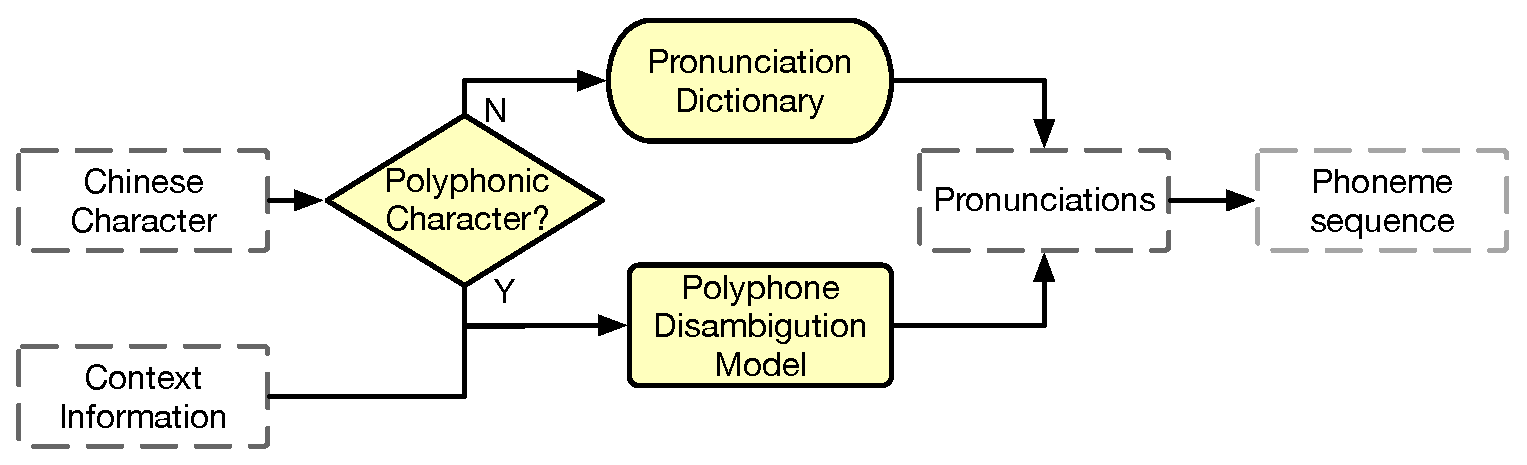
\includegraphics[width=8cm]{pics/ChineseG2P.eps}}
		%  \vspace{2.0cm}
	\end{minipage}
	\caption{Chinese G2P Flow}
	\label{fig:model-framework}
\end{figure}



For polyphones in Chinese, their pronunciations are affected by two factors, tonal modification and semantics. \cite{lilinhui2010} When two or more syllables are combined, the syllable value sometimes changes and is different from the single utterance, which is tonal modification. Because the tonal modification can be postponed to the later speech generation stage, the main focus is homographs affected by semantics in G2P stage.

The earliest system was based on manual rules for Chinese homograph disambiguation.\cite{dajunzhang2000, lianhongcai1995} The linguistic experts summed up the laws of homograph disambiguation and wrote these rules into computer-understandable forms. However, as the number of rules increases, the environment of a polyphonic character may be matched by multiple rules. Rule conflicts are difficult to avoid. This is one of the main problems that is difficult to solve based on the rule method. As the amount of data increases, more and more people try to use statistical approaches for homograph disambiguation.
As the amount of data increases, more and more researchers try to use statistical approaches for homograph disambiguation. Decision trees were applied in \cite{wang1996broad} to classify the pronunciations of homographs. A study in \cite{fangzhouliu2007} has shown that a Maxent model outperforms decision tree in homograph disambiguation. But these statistical approaches need handcrafted features extracted for the polyphonic character as input, the process of feature extraction can be cumbersome and requires some linguistic knowledge.

Deep neural network (DNN), which can learn high-level invariant features from raw data \cite{bengio2013representation}, provides an easier way to extract valid features and predict the pronunciation of polyphonic character. Shan et al. \cite{shan2016bi} address the polyphone disambiguation problem as a sequential labeling task, propose to use bidirectional long short-term memory (BLSTM) neural network to encode the polyphonic character’s surrounding observations as its inputs and predict the pronunciations. This LSTM approach eliminate the process of extracting handcraft features though still needs to use the word segmentation tool to preprocess the text, and its prediction accuracy outperform the max entropy method.

In this paper, we propose an end-to-end approach for Chinese homograph disambiguation based on pretrained BERT \cite{devlin2018bert}. Our model consists of two parts, BERT and DNN classifier. The BERT is pretrained using two novel unsupervised prediction tasks: to predict the masked part of input and to predict the next sentence. So the BERT is expected to extract the features containing semantic information, the following DNN classifiers these features to predict the pronunciations of polyphonic characters. Our model accepts only raw character sequence and the index of polyphonic character as input removing the preprocessing steps used by all the other methods. Experiments shows our proposed method outperform the LSTM baseline over 1\% on overall accuracy on our experimental settings.

\section{The proposed approach}

\begin{figure}[t]
	\centering
	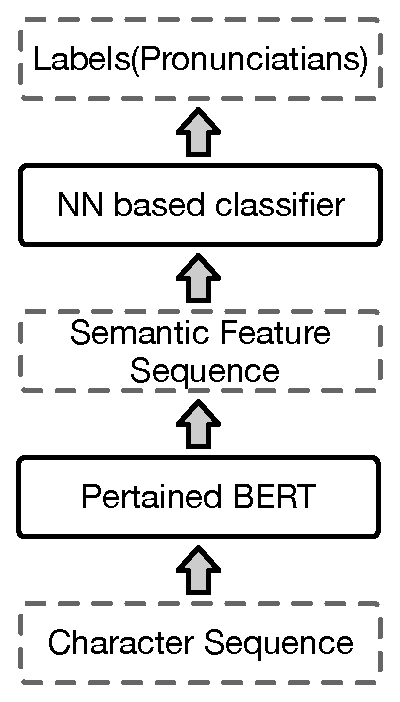
\includegraphics[scale=0.4]{pics/architecture2.eps}
	\caption{Model architecture}
	\label{fig:model_architecture}
\end{figure}

Fig.\ref{fig:model_architecture} depicts the architecture of our model, which consists of two parts, a pretrained BERT and a classifier based on neural network (NN). The pretrained BERT extracts features containing semantic information from a sequence of Chinese character, and the NN based classifier predicts all the possible pronunciations of all the polyphones according to the extracted semantic feature sequence.


\subsection{Model detail of BERT}

\begin{figure}[t]
	\centering
	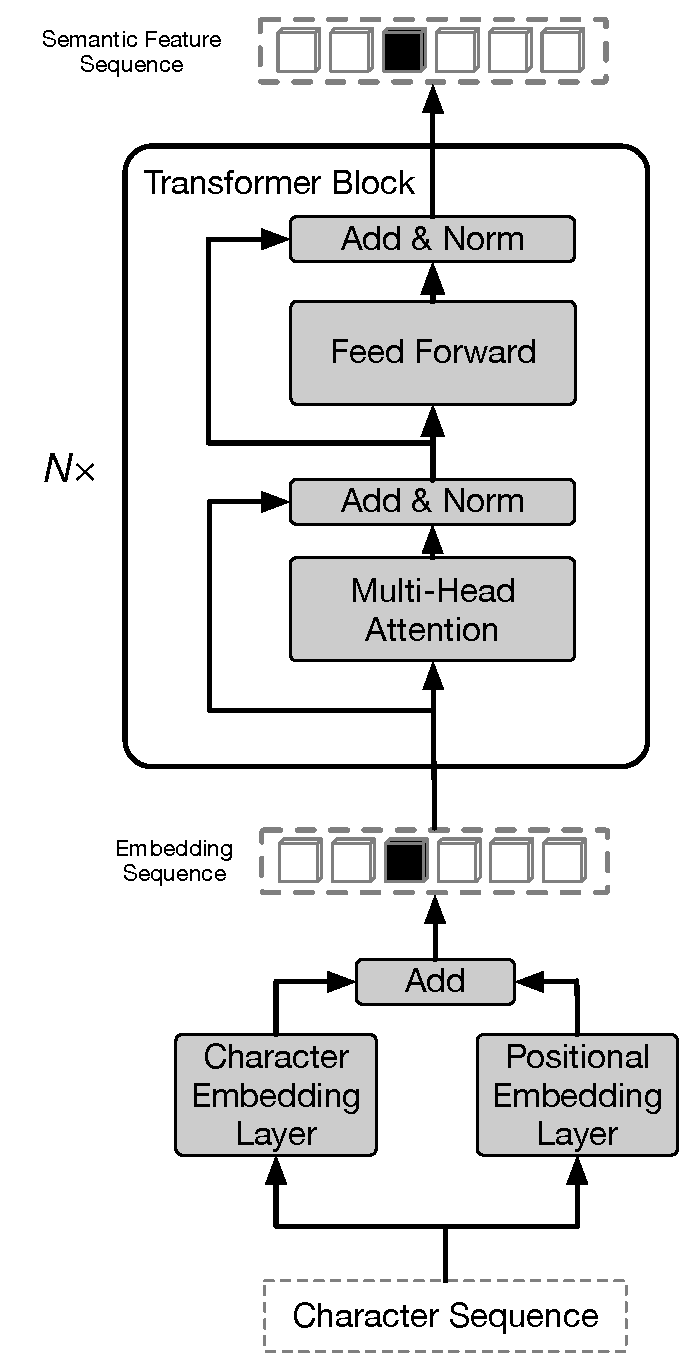
\includegraphics[scale=0.4]{pics/bert2.eps}
	\caption{BERT architecture}
	\label{fig:bert}
\end{figure}

As shown in fig.\ref{fig:bert}, the BERT accepts sentence containing polyphone in the form of Chinese character sequence as input, and extracts semantic feature sequence corresponding to the input sentence.  The character sequence is processed by character embedding layer and positional embedding layer respectively, then the resulting character embedding and positional embedding are add together to feed the following stacked transformer blocks. The transformer block mainly consists of two parts, multi-head self-attention mechanism and position-wise fully connected feed-forward network.

During pretraining phase, the BERT model is pretrained with two predict task, predicting the masked input characters and predicting the next sentence. So the pretrained BERT model is expected to extract semantic representing from raw character sequence.


\subsection{Model detail of NN based classifier}

\begin{figure*}[htbp]
	\begin{minipage}[t]{0.3\linewidth}
		\centering
		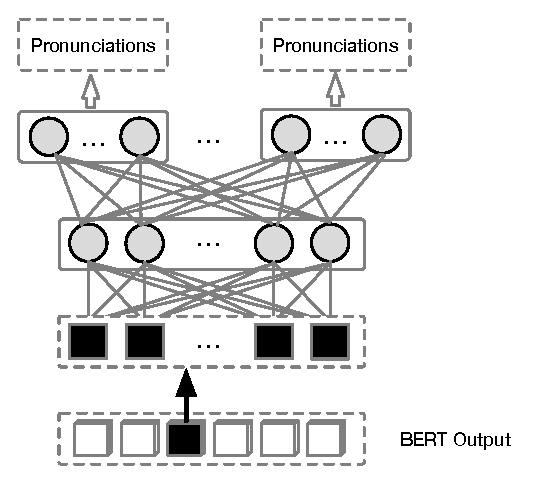
\includegraphics[width=2.0in]{pics/FC2.eps}
		\caption{fig1}
		\label{fig:side:a}
	\end{minipage}%
	\begin{minipage}[t]{0.3\linewidth}
		\centering
		\includegraphics[width=2.0in]{pics/lstm2.eps}
		\caption{fig2}
	\end{minipage}
	\begin{minipage}[t]{0.3\linewidth}
		\centering
		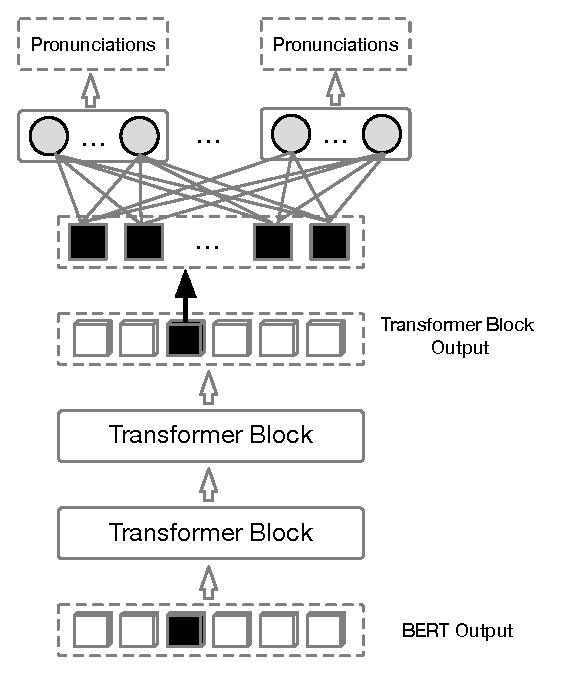
\includegraphics[width=2.0in]{pics/sa2.eps}
		\caption{fig2}
		\label{}
	\end{minipage}
\end{figure*}

\subsubsection{Fully connected feed-forward network based classifier}

As BERT model is pretrained with the task to predict the mask characters and the next sentence, it is reasonable to expect that the extracted features contain semantic information. As the pronunciation of polyphone is decided by semantics, a natural idea is to predict pronunciation of polyphone according to the corresponding semantic feature extracted by pretrained BERT.

Fig.\ref{fig:mlp} depicts the model structure of classifier based on fully connected feed-forward network. It accepts the semantic feature corresponding to polyphone as input, if polyphone is the $i$th element of the bert input character sequence, the semantic feature corresponding to polyphone is the $i$th element of the bert output feature sequence. The classifier consists of two fully-connected layers, and the size of the last full-connect layer is equal to the number of all the possible pronunciation of all the considering polyphones. That's mean, we predicted the pronunciation of all the polyphone with one neural network model. During the training phrase, there is a dropout layer between the fully-connected layers.

\begin{figure}[t]
	\centering
	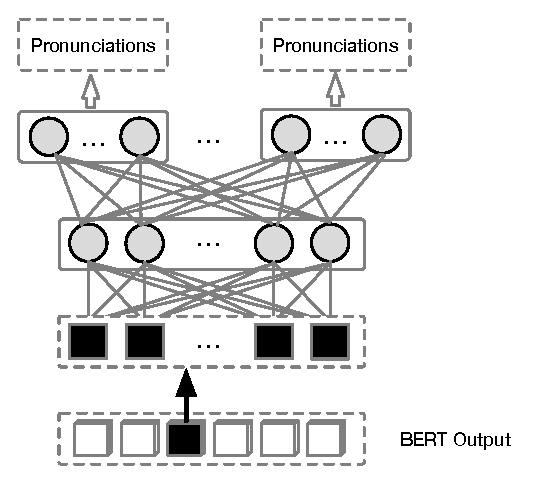
\includegraphics[scale=0.5]{pics/FC2.eps}
	\caption{MLP based classifier}
	\label{fig:mlp}
\end{figure}

\subsubsection{LSTM based classifier}
\label{sssec: lstm_based_classifier}

Indicated by [10], contextual information such as the POS of polyphone's neighbor words can also affect the pronunciation of polyphone. So instead of using the semantic feature corresponding to polyphone to classify directly, using BLSTM to model the contextual information before classifing may be a better choice.

As shown in fig.\ref{fig:lstm}, the semantic feature sequence is processed by a two-layer BLSTM network, then a dense layer project the element in output sequence corresponding to polyphone to the number of all the possible pronunciations of all the considering polyphone.

\begin{figure}[t]
	\centering
	\includegraphics[scale=0.5]{pics/lstm2.eps}
	\caption{LSTM based classifier}
	\label{fig:lstm}
\end{figure}

\subsubsection{Transformer block based classifier}

Due to the characteristics of the recurrent network, the output element of BLSTM corresponding to polyphone focuses more on the neighboring, to better model the long-term dependence, we use transformer block replace lstm in \ref{sssec: lstm_based_classifier}, depicted in fig.\ref{fig:sa}

\begin{figure}[t]
	\centering
	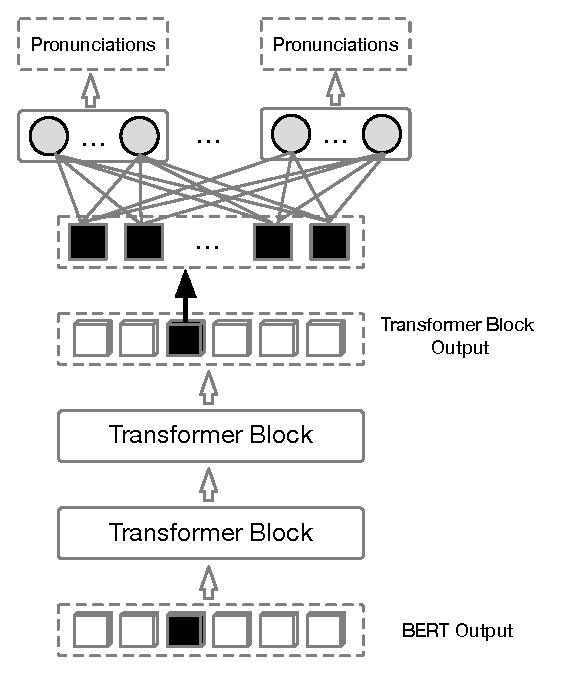
\includegraphics[scale=0.5]{pics/sa2.eps}
	\caption{Transformer block based classifier}
	\label{fig:sa}
\end{figure}

\section{Experiment and analysis}

\subsection{Experimental setup}

The dataset is extract from TTS corpus in Tencent AI Lab, all the polyphone appears 331325 times. In our following experiments, we only consider polyphone which appears more than 2000 times, a toal of 29 such polyphones and 134 possible pronuciations. The total appear time of these 29 polyphones is 277450, 83,7\% of the total appeartimes. The number of predict labels is 135, one more represents other pronunciation. The dataset is divided into 10 subsets randomly, and we conducted 10-fold cross-validation to get the final result. 

\subsection{Setting of baseline method}

In baseline LSTM-based polyphone disambiguationmethod, First of all, word segmentation and POS tagging is processed on input character sequence, then we put the word containing the polyphonic character as the center of the word sequence and consider the word's left and right neibhboring words as context, meanwhile we get a corresponding POS sequence. We split the center word containing polyphonic into character level, and mask the neighboring word as zero. meanwhile, we duplicate the center of POS sequence several times corresponding to the splitting of the center word in word sequence.

Fig.\ref{fig:lstm_baseline} shows the flow digram of the baseline LSTM-based polyphone disambiguation method. tagging pronuciation is viewed as a sequence labeling problem. The label in output sequence not corresponding to polyphonic character is expected as "the other". The pos embedding is trainable, and the word embedding use pretrained embedding dict provided by [9]. The hidden size of LSTM is 512, and the context words number to be consider is 1 as described in [7]. 


\begin{figure}[t]
	\centering
	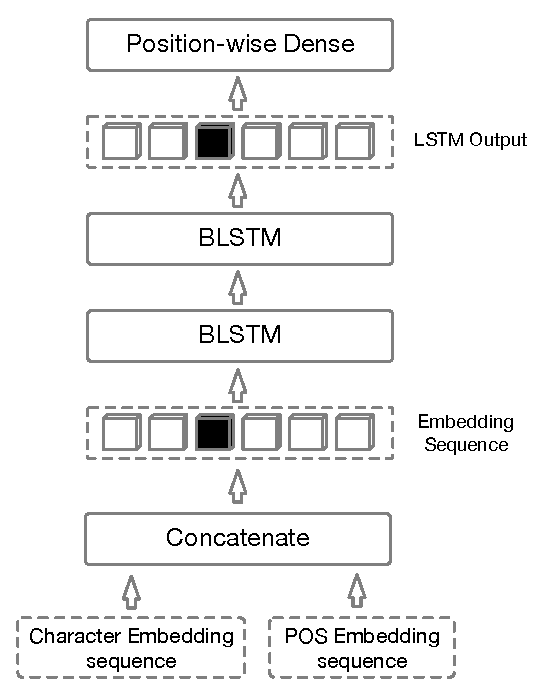
\includegraphics[scale=0.5]{pics/lstmbaseline2.eps}
	\caption{LSTM approach for polyphone disambiguation}
	\label{fig:lstm_baseline}
\end{figure}

\subsection{Setting of the proposed method}

\subsection{Experimental result}

\begin{table}[th]
	\caption{The result}
	\label{tab:example}
	\centering
	\begin{tabular}{ r@{}l  r }
		\toprule
		\multicolumn{2}{c}{\textbf{Method}} & 
		\multicolumn{1}{c}{\textbf{Accuracy}} \\
		\midrule
		Baseline&  & 0.931            \\
		BERT + FC  &                     & 0.947               \\
		BERT + LSTM &                     & 0.956       \\
		BERT + Transformer block&      & 0.954             \\
		%    $10$                      & $/1$  & $20$~~~              \\
		%    $100$                     & $/1$  & $40$~~~              \\
		%    $1000$                    & $/1$  & $60$~~~              \\
		\bottomrule
		\end{tabular}
		
	\end{table}



\subsection{Analysis}





\section{Conclusions}




\bibliographystyle{IEEEtran}

\bibliography{mybib}


\end{document}
